\chapter{Investigation Models \TODO}
\setlength{\epigraphwidth}{3in}
\epigraph{By failing to prepare, you are preparing to fail}{Benjamin Franklin}

This chapter continues the introduction of technical privacy
auditing by introducing the Technical Privacy Auditing Model and
previewing three examples of how the model will be applied to
different kinds of data later in this book.

\section{The Technical Privacy Auditing Model \TODO}

\begin{enumerate}
\item \textbf{TARGET} Determine the systems or data objects to examine.
\item \textbf{RESEARCH} Find information about the data formats in
  questions and the tools that are available to analyze them. 
\item \textbf{COLLECT} Obtain exemplars, ideally from multiple instances.
\item \textbf{ANALYZE} Extract Features; Look for oddities and outliers
\item \textbf{EXPERIMENT} Show that you understand what is happening
\item \textbf{REPLICATE} Ideally on another system
\item \textbf{REPORT} Share results in a concise \& understandable form
\end{enumerate}


\subsection{Applying the model redacted PDFs \TODO}

\subsection{Applying the model to JPEGs \TODO}

\subsection{Applying the model to network traffic \TODO}

\section{The Digital Forensics Model \TODO}

Even though every case is different, DF practitioners have developed an
approach to conducting investigations called the 
\emph{digital forensics model}\cite{pollitt:models}. The 
elements of the model include:

\begin{description}
\item[Preparation] Before performing an investigation, those involved
  must prepare themselves by deciding upon the standards and
  procedures that will be followed; receiving the necessary training;
  and obtaining the appropriate equipment and software required for
  investigations. 

  To use the example of the cell phone from above,
  preparation may involve obtaining specialized hardware that can extract the
  memory from a cell phone and practicing one's technique on phones that are not part
  of the investigation.

\item[Collection and Preservation]
  Before data can be analyzed, they   must be removed from the
  device being analyzed and preserved to create a lasting
  record. Without this step, it may not be possible to repeat an
  analysis at a later point in time. 

  In our example, this step might involve the actual extraction of data
  from the cell phone into a single file called a \emph{physical
    image} that records all of the phone's applications, phone data, user data,
  and deleted files. Such a physical image might be 64GB in size or
  even larger.

\item[Examination and Extraction] Working with the preserved data, an
  examiner will explore for any information that might be
  relevant to the investigation at hand. Once that information is
  found, it is extracted and isolated.

  In our example, this step might involve the extraction of each
  digital photograph from the \emph{physical image} and the storage of
  each photograph in its own file. The files might be named according
  to where they were found in the physical image (e.g. 62071808.jpg)
  rather than with the name that they were given by the phone
  (e.g. IMG001.JPG). The examiner might also extract \emph{metadata}
  from each photograph such as the time and GPS coordinates associated
  with each exposure and the serial number of the camera that took the
  photograph. This information might be stored in a separate file for
  each photograph (e.g. 62071808.txt) or might be stored in a single
  spreadsheet for all of the photographs (e.g. jpeg-metadata.xls).

\item[Analysis] Once the specific data being analyzed has been
  extracted, the analyst will construct one or more hypotheses that
  uses the digital evidence to explain possible past activities. A
  hypothesis may draw from multiple digital devices---an email message
  sent from a desktop computer to a cell phone, for example---or the
  hypothesis may incorporate events in the physical world, like a
  power failure or theft. During this phase a good analyst will also
  try to construct alternative hypotheses that are consistent with the
  evidence but which point to different conclusions. 

  In our example, the hypothesis may be that a specific photograph was
  taken with the phone in question. This may be supported by the
  photograph having similar metadata to a photograph taken a few
  minutes earlier or later. An alternative hypothesis may be that the
  photograph was downloaded to the phone over a network.

\item[Reporting and Testimony] Finally, the analyst will
  produce a written report or give testimony in a courtroom.
  Judges and juries can't examine digital evidence for
  themselves---even if they had the training and the technical skills
  to do so, performing their own analysis would be inappropriate:
  their role in the legal process is to evaluate the law, the evidence
  and make a legal determination, not to perform technical
  analysis. Reports and testimony must therefore be 
  \emph{complete}---they must describe the tools and procedures
  that were followed, clearly document what was found, and then
  separately provide the technical interpretation of the
  evidence. 

  In our example, the analyst might prepare a report documenting how
  the phone's contents were copied, the tools that were used to
  extract the photographs and their corresponding metadata, and how
  the evidence is consistent with the analyst's hypothesis. 

\end{description}

The model brings reliability and repeatability to the process, helping
to assure that different examiners working with the same data will
arrive at the same conclusion. 

Because they can look into the past and uncover hidden data, DF tools
are increasingly used beyond the courtroom. Security professionals use
DF tools to analyze network intrusions---not to convict the attacker,
but to understand how the attacker gained access to plug the
hole. Data recovery firms use DF tools to resurrect files from drives
that have been inadvertently formatted or damaged. 

Forensic tools are also used to determine that something did not
happen. Here they are less powerful, for the well known reason that
the absence of evidence is not the evidence of absence. 
For example, in May 2006 a laptop and external hard drive containing
sensitive personal information of 26.5 million veterans and military
personnel was stolen from an employee at the Department of Veterans
Affairs. After the stolen laptop was recovered in June 2006, forensic
investigators analyzed the media and determined that the sensitive
files had probably not been accessed\cite{va-laptop-1}. One way to
make such a determination is by examining the access and modification
times associated with each file on the computer's hard
drive. Of course, the same
forensic techniques that the investigators used could have been
applied to access the VA laptop without modifying those timestamps,
the VA investigators really just determined that the files had not
been asked by convention, non-forensic means.

As the preceding paragraphs make clear, today the field of digital
forensics is largely \emph{tool-based} and
\emph{investigator-centric}. 
That is, the requirements of DF are driven 
by what investigators need to perform digital
investigations\citep{walls-levine-effective-digital-forensics}. Convictions
are frequently the
measure of success. In many cases there is a considerable gap between
what is theoretically possible and what is necessary. That is, even
though there may be an intellectual desire to analyze and explain every last byte
on a piece of subject media\cite{garfinkel:every-last-byte}, there is
rarely a reason to do so.

\subsection{Fraud Detection in Multimedia}

Even when photos and video can be recovered from a subject's computer
or cell phone, another question to consider is whether or not the
imagery is real. Photographs were doctored long before the advent of
PhotoShop. For example, after he was purged by Stalin, Abel
Yenukidze was carefully removed from official photographs through a
series of skillful manipulations of light and negatives in a Kremlin darkroom\citet{stalins-darkroom}. Today
computer animation takes such manipulation to a completely new level,
with computers now able to synthesize scenes that are 
indistinguishable from recorded reality (\figref{ultra-realistic}). 

\begin{figure}
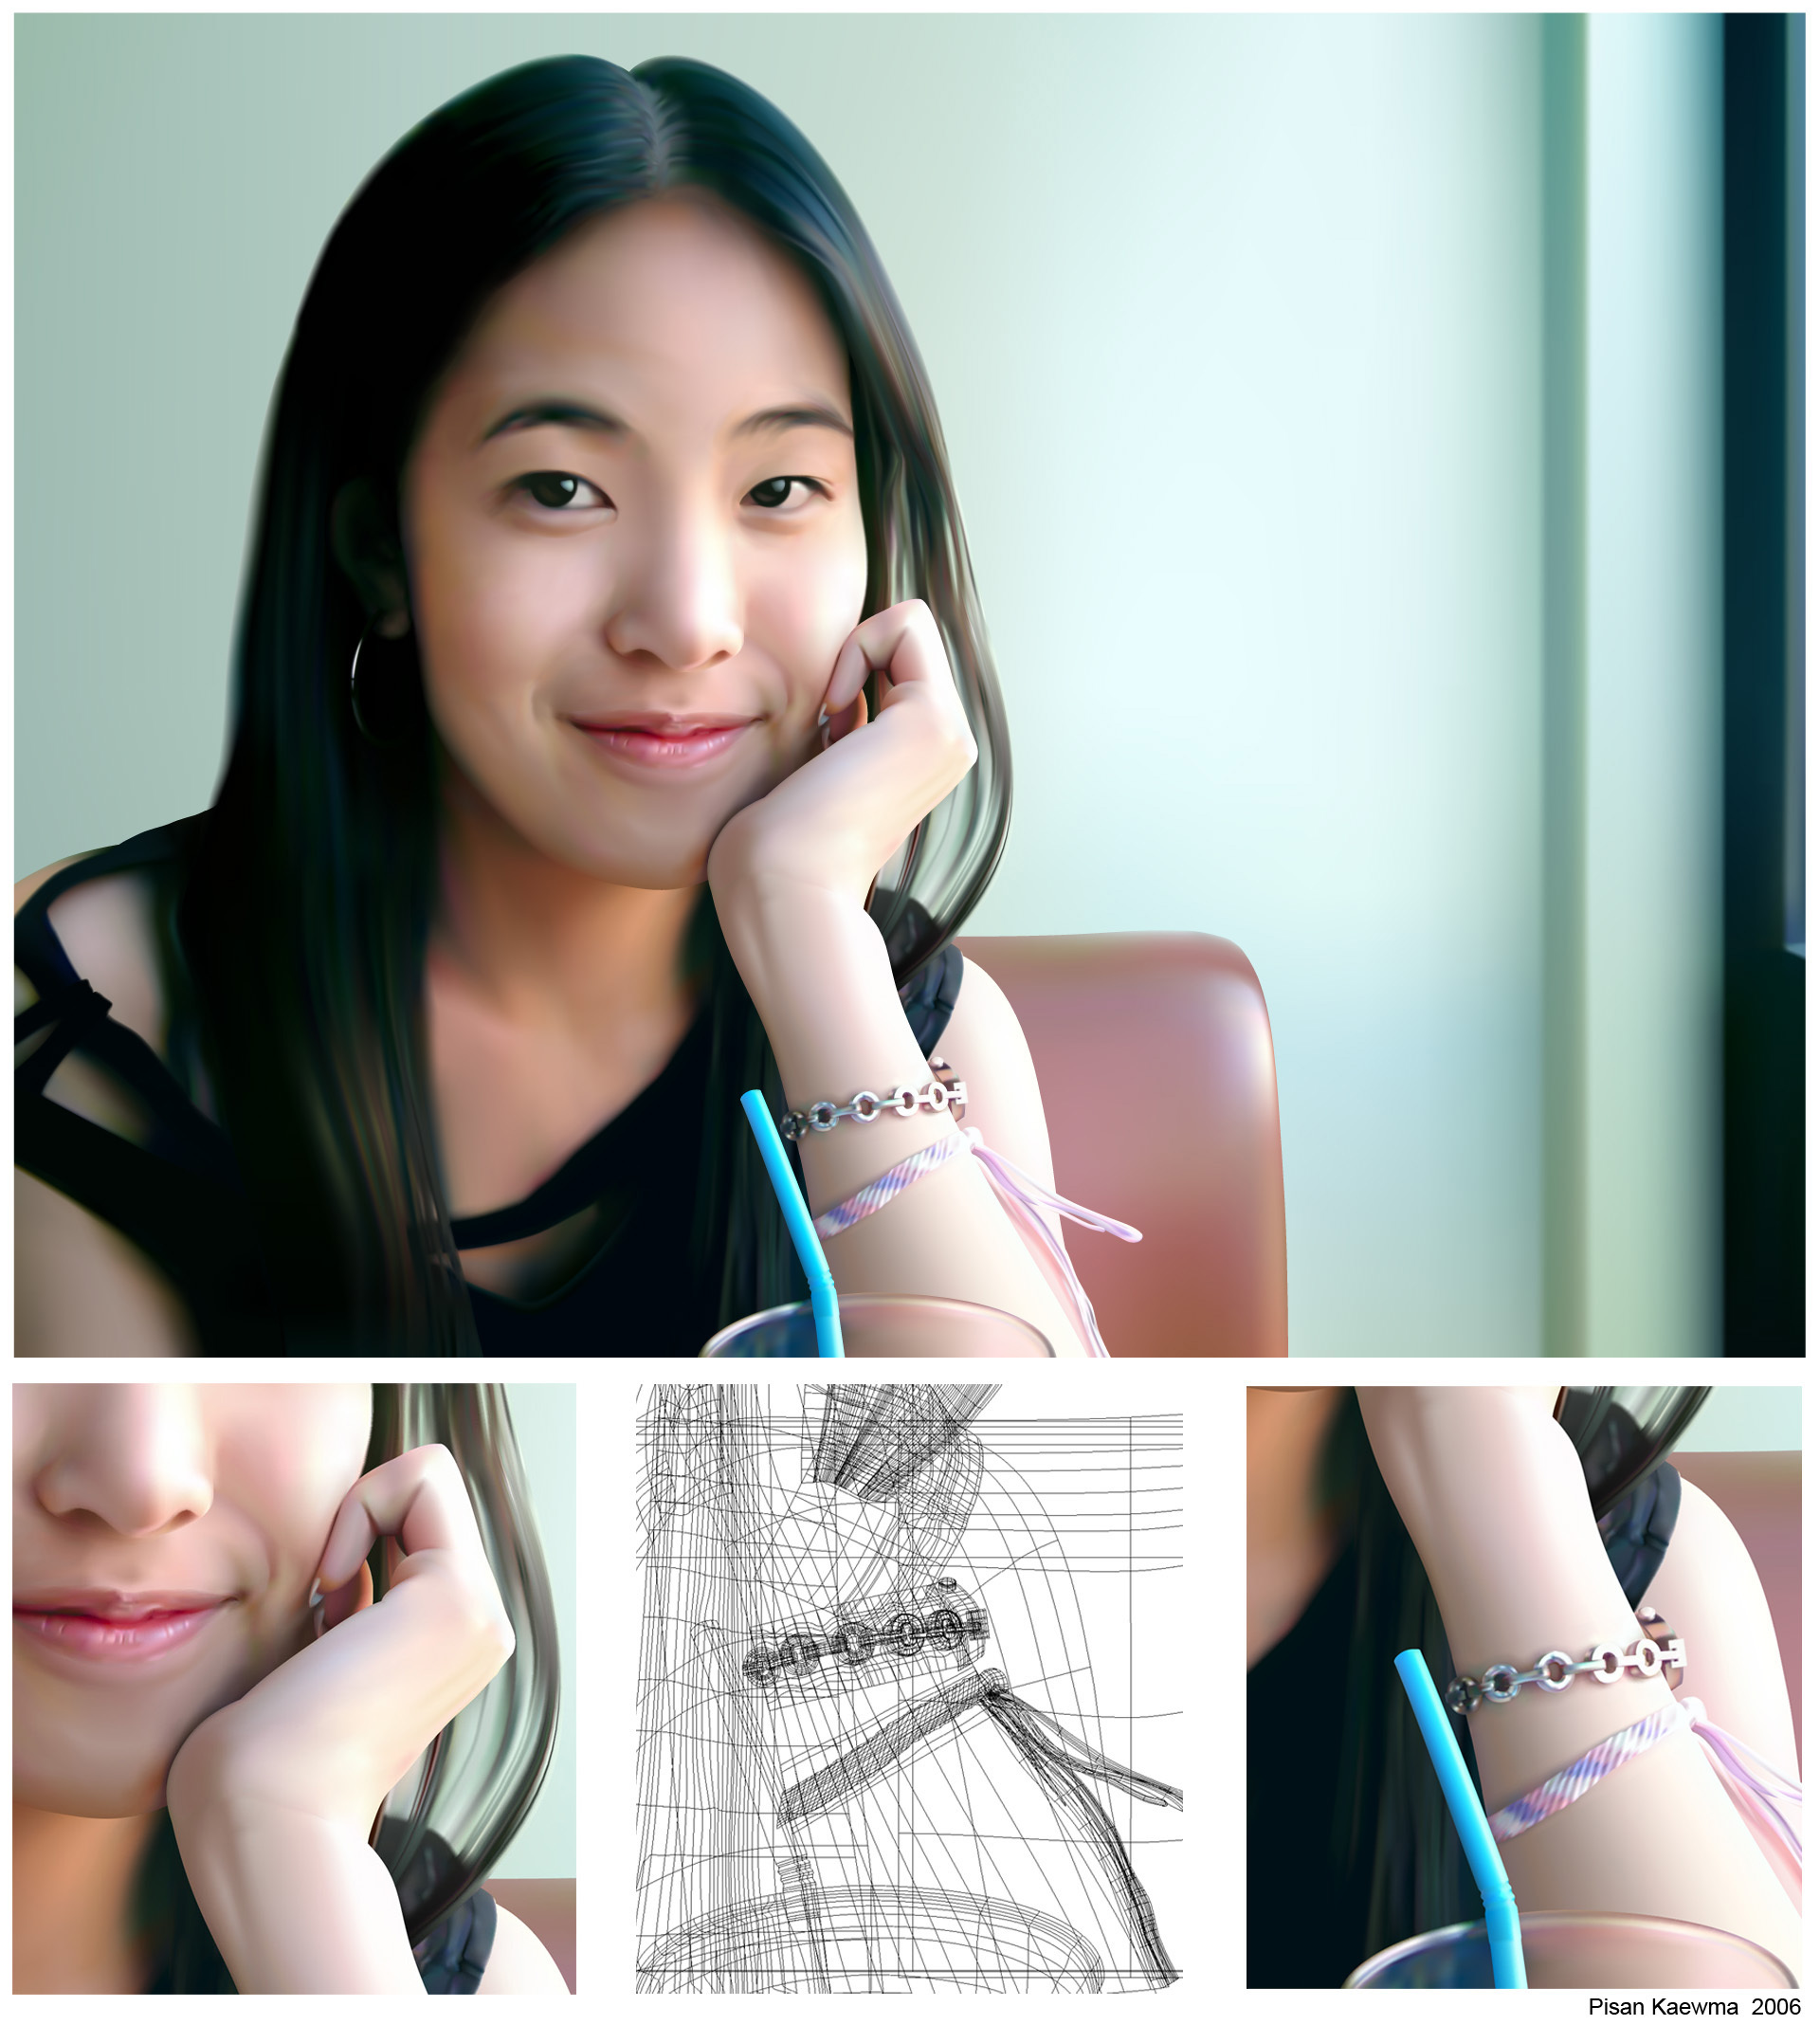
\includegraphics[width=4in]{art/a1336.jpg}
\caption{Ultra realistic vector gradient mesh using Adobe Illustrator by Pisan Kaewma, Thailand}\label{ultra-realistic}
% http://10steps.sg/inspirations/artworks/photo-realistic-vectors/
% http://www.ebypaidrick.com/Gallery.html
% http://www.illustratorworld.com/artwork/1336/
% http://rcpopart.com/labels/hyper-realist%20sculptor.html
% http://www.real-trace.com/index.html
\end{figure}

Recent developments in image processing have made it
possible to find some kinds of artifacts that indicate tampering or wholesale synthesis. For example,
the JPEG compression algorithm produces a mathematical signature when an
image is decompressed, cropped, and then re-compressed. Specular 
reflection, highlights and shadows can be closely examined to reveal
that different objects in a single ``photograph'' actually were
assembled from objects that were in 
slightly different physical environments. In one particular dramatic
demonstration, Dr.\ Hany Farid of Dartmouth University showed that a single ``group picture''
had been created by pasting in the people from different photos
because the reflection of the room lights on each person's eyeballs
were inconsistent with were they were standing in the frame. The technology is now
being commercialized\citep{farid07}.


\section{Digital Forensics Challenges \TODO}

For all of its power, DF practitioners face stark
challenges in practicing their discipline---challenges likely to
increase in the coming years. Those challenges are size,
time, diversity, cloud computing, encryption and language.

\begin{description}

\item[Size:] The past three decades have seen a steady increase in the
  amount of storage available to consumers and a steady decline in its
  cost. In 1993 I purchased my first 1 gigabyte external hard drive
  for a thousand dollars; today a 1 terabyte external hard drive can
  be purchased for under a hundred---a thousand times more
  storage for a tenth the price. Not surprisingly, the amount of data
  acquired by law enforcement organizations in their cases is
  increasing every year.

  Alarmingly, other aspects of computing have not scaled as quickly as
  storage. Today's terabyte drives are only 10 to 100 times faster
  than the gigabyte drives of yesteryear, which means that it takes anywhere
  from 10 to 100 times longer to copy  data from the larger
  drives. Likewise, today's computers are only on average 100 fold
  faster than the high-end workstations of the early 1990s, which
  means that there is less computing power available to process each
  byte per unit time. The continuation of these trends means that new techniques are
  required to deal with the data onslaught, as existing techniques
  simply cannot keep up with the increased storage available to consumers.

% My 33Mhz NeXTstation had 10 SPECmarks
% http://www.kevra.org/TheBestOfNext/NeXTProducts/NeXTHardware/NeXTStnColor/files/page620_2.pdf
% Intel Core i7 is 965 SPECmarks
% http://openlab.web.cern.ch/sites/openlab.web.cern.ch/files/technical_documents/CERN_openlab_report-Eval-of-energy-consumption-and-perf-of-Intel's-Nehalem-achitecture.pdf

\item[Time:] Even as the amount of storage received by law enforcement
  organizations increases, the time available to analyze that storage
  is steadily decreasing. In part this is because the number of cases
  in which digital evidence is collected is increasing far faster than
  the number of forensic investigators available to do the
  examinations. But another cause is the increasing realization that
  DF can be used to \emph{solve crimes}---that is, as
  part of the investigation process---whereas in the
  past DF was mainly a tool for \emph{assisting in convictions}. The
  shortened time horizons puts increased demands on tools,
  investigators, and systems.

\item[Diversity:] Forensic investigators must be able to process any
  information found on any computer system currently in use. After
  all, if there were a particular kind of system that could not be
  analyzed, criminals would be sure to use it. Thus, DF tools and
  invesitgators must be able to accommodate all kinds of computers,
  operating systems, application programs and the like. The diversity
  is particularly problematic in the case of cell phones, where there
  are literally dozens of different kinds of cables and tens of
  thousands of apps in widespread use that might require analysis.

\item[Cloud Computing:] Further complicating the investigator's job is
  the emergence of cloud computing and other technologies for storing
  data in the Internet rather than on desktops, laptops, and mobile
  devices. As a result of the cloud, there is no way to assure that a
  seized cell phone actually holds the suspect's data---the phone
  might simply be a tool for accessing a remote server. A law
  enforcement professional who is authorized to search a device may
  not have legal authority to use information on that device to access
  remotely stored data. Worse still, the data might be deleted in the
  meantime by one of the suspect's collaborators.

\item[Encryption:] The increased use of encryption means that
  investigators might not be able to decipher information once they
  have it in their possession. 

\item[Language:] Finally, in today's global environment forensics
  examiners are increasingly encountering evidence written in human
  languages that the examiner does not understand. And while tools
  like Systrans and Google Language Tools can perform some automated
  language translation, such systems are rarely sufficient for
  real-world forensic media.

\end{description}

